\chapter{Mycelium Machine \& Materials}


\section{Overview}

This projects aim to develop an easy way to make mycelium-based biocompisites. We present two similar Controlled Environment systems for mycelium based composite that can be developed easily with DIY and low cost hardware.
One of this project focus more on monitoring un data management, the other one is mare about modularity and transport 
In both cases, we're talking about controlled-environment systems with a closed space, thermal resistance or heating mats, temperature sensors, humidity modulators and associated relative humidity sensors, carbon dioxide sensors and fans for air renewal and circulation. 
And of course a control and data transmission system. 

% \begin{figure}[h]
%     \centering
%     \includegraphics{images/Myceliummachine.png}
%     \caption{System design representation}
%     \label{fig:}
% \end{figure} 

\section{Systems design}

The controlled Environment systems takes the form of a closed box, isolated from external climatic conditions. this box is where the inoculated substrate for mycelium growth is placed: “Mycelium grow space”. 
The Mycelium grow space is instrumented with climate sensors. in this case a relative humidity sensor, a temperature sensor and a carbon dioxide sensor. they are connected to an ESP-type microcontroller which handles data reading.
The ESP will then send the data via an MQTT protocol to a RaspberryPI acting as an MQTT broker and server for an Influx database. The data can then be visualized via a dashboard on a user's computer. 

On the ESP, a main user can select the desired climate variables. This will change the conditions according to which the microcontroller will activate or deactivate relays. This will switch on or off climatic actuators (ie: thermal resistance etc...) which will also change the internal climatic conditions in the space.  
Everything will act automatically once the variables have been chosen by the user (Automation loop). 

This architecture allows the simultaneous use of several controlled environments with different growth conditions. Users can choose, via the MQTT protocol, whether or not to subscribe to a controlled environment and see the data associated with it. 

\begin{figure}[h]
    \centering
    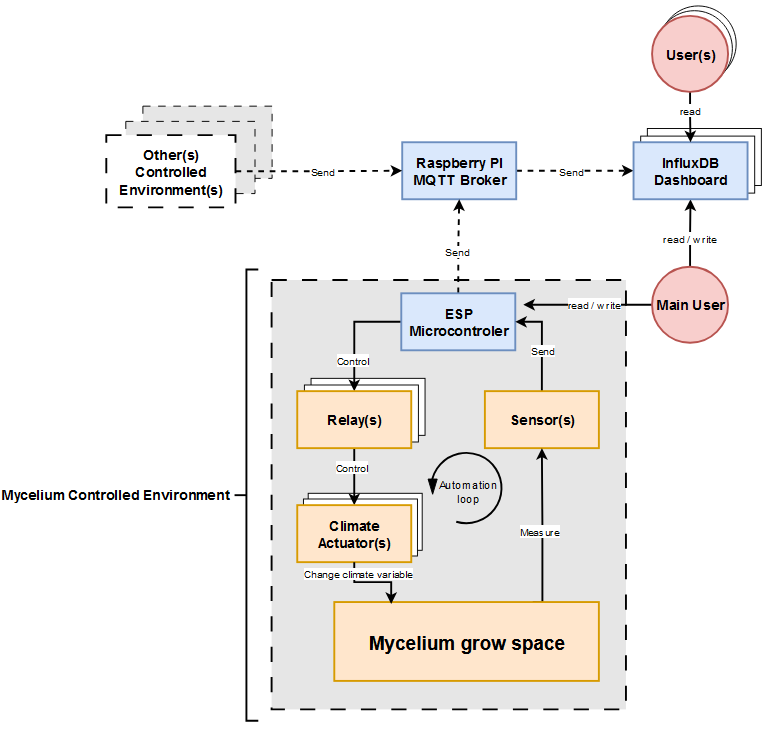
\includegraphics[width=1.4\textwidth]{images/diagMyceliummachine2.png}
    \caption{System design representation}
    \label{fig:blasttrash}
\end{figure} 


\section{Manufacturing Processes \& Grow Theory}

In a natural environment, the mycelium grows in the soil in search of nutrients. when it emerges from the soil into the air or under leaves, it is still in an environment rich in carbon dioxide. at this point, the mushroom stem (fruit of the mycelium) will grow until it reaches the air with more oxygen and forms the mushroom cap. 

In the case of Mycelium-based biocomposite, the mycelium will be innoculated in a substrate rich in nutrients and/or fibrous material. 

As explained above, the mycelium will agglomerate the substrate, greatly increasing the solidity of the innoculated substrate compared with the solidity prior to growth. 
When the mycelium comes into contact with the substrate in an oxygen-rich environment, it will blach and form a hydrophobic, fireproof layer.
That is why control carbon dioxide concentration is very important for mycelium material

Air renewal is also important for two other reasons: on the one hand, mushrooms breathe like we do, so they consume oxygen and spit out carbon dioxide. So the carbon dioxide concentration in the closed enclosure increases over time. Without air renewal, the mycelium will eventually aphyxiate itself. 
On the other hand, air renewal reduces the appearance and development of other pathogens or molds that would compete with the mycelium, and thus reduce its development. 


\paragraph[short]{Manufacturin Processes}

The approach is very similar to the literature described above \ref{Fab_process}.
first, the substrate is sterilized. then mycelium is mixed with the substrate in molds and placed in the controlled Environment for two or three weeks. 

During growth, once the mycelium has grown enough that the inoculated substrate no longer needs to be in the mold for growth. 
Then the molds are carefully removed to allow the mycelium to breathe as much as possible, especially on the surfaces in contact with the mold. 

After the growing phase, the Mycelium based biocompisites are dried in an oven for a minimum of 5 hours, depending on size or thickness, at a maximum of 80°C. 

\section{Contribution}

\subsection{Environment controlled}

The project consists of 3 main sections: the mycelium growth area, the water tank and the electrical panel.

The mycelium-growing part is a plastic box of around 100 liters, with its walls lined with bubble-wrap to provide thermal and light insulation. The box has also been modified by adding elastics to create tiers in the box to accommodate the molds and ensure uniform air circulation. The box houses the sensors directly connected to the electric panel and also houses thermal resistance. This section has 3 pipes. 2 for the air inlet and outlet sent by the filter fans, and one connected to the water tank.

The water tank consists of a water box containing a fogger and a centrifugal fan, both of which are connected to the electrical panel. There is an air inlet and an air outlet. The fan is located at the air inlet, while the air outlet is connected by a pipe to the growth space.

The fogger is immersed in the water in the reservoir. When the fogger and fan are switched on, the fogger will create an aerosol of water which will be transported to the growth space via the air flow created by the fan. This will increase the humidity in the growth space.

The electrical panel manages all the electrical or electronic parts of the project. In other words, the power supply, the microcontroller and the relays that control the various climatic actuators. The electrical panel is connected via a mains socket to power the entire system.

Everything was placed on a large board overlaid with wheels for ease of movement. 

\begin{figure}[h]
    \centering
    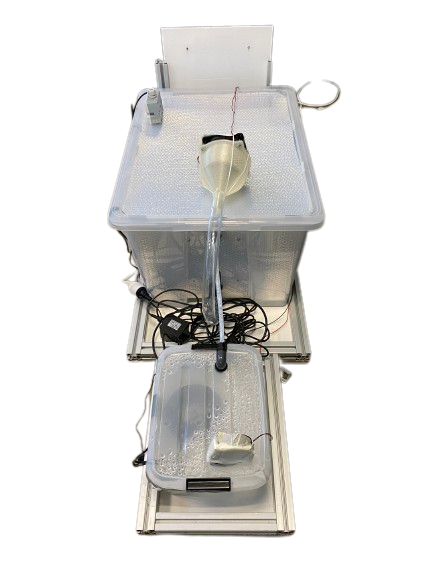
\includegraphics{images/myceliummachine.png}
    \caption{Environment controlled for mycelium picture}
    \label{fig:Mycemachinne}
\end{figure} 


The mycelium used was ganoderma lucidum, also known as reishi, the most widely used mushroom in the literature.\cite{yang2021material}
Moreover, this mushroom seems to have better mechanical properties, even if it seems that it's mainly the subtrate that dominates over the mechanical properties. 

Several types of substrate have been tested. More fibrous substrates such as coconut fiber. More granular substrates such as corn husks. Nutrient-rich substrates such as coffee grounds. Low-organic substrates composed mainly of minerals. 
And combination mixes of its substrates.

In addition, the direction of the fibers in the substrate also affects the mechanical properties. In other word fibrous substrates may have greater mechanical properties or the opposite, depending on how they were placed in the substrate.

\paragraph{Software}

There are 2 programs for the project. the program on the esp that reads the data, activates or deactivates the relays, and sends the data to the servers on the rasberry. 
And the program on the raspberry which receives the data and displays it via a dashboard in an influxDB database. 

On the ESP, the main user chooses the climatic variables for activating and deactivating the climatic actuator. In other words, the user chooses the climatic variables in which the system will be located. For example, for relative humidity, if the user chooses that the environment to be controlled should be between 80\% and 90\% humidity. Then when the humidity sensor reads that the humidity is below 80\%, ESP will activate (via the relays) the climatic actuators responsible for humidity control, i.e. the fogger and fan. Afterwards, ESP will deactivate the actuators once the sensor returns a humidity above 90\%.

It will be the same for the control of other climatic variables. 

In pallalele, the data read by the sensors will be sent via MQTT to an influx database on hermger on a raspberry. 
Influxdb is a database management system. in particular, it can be used to create dashboards, which can be used to monitor sensor data directly from a computer connected to the database. 

\begin{figure}[h]
    \centering
    \includegraphics{images/laptopdashboard.png}
    \caption{dashboard of mycelium controlled environent}
    \label{fig:Mycemachinne}
\end{figure} 

\paragraph{Hardware}

In material terms, the system can be divided into several categories of subsystems. 
Each subsystem is made up of several parts that perform the same type of function (measuring, controlling, managing climatic conditions...). 

\textbf{The climatic actuators} 

The climatic actuators are among the most important parts of the system, as they determine the climatic conditions in the growth chamber. 

The relative humidity control system consists of two parts: a fogger and a centrifugal fan,both located in the water tank. 
The fogger is placed directly in the water; when switched on, it vibrates a ceramic cell, producing a fog on the surface of the water. 
When the centrifugal fan is switched on, it will create a flow of air changed from the fog created by the fogger, which will come out of the water tank through a pipe connected to the growth chamber, increasing the humidity in the space. 

To increase humidity in the growth chamber. The choice of the fogger and the centifugal fan is justified by their simplicity of implementation. In fact, the fogger's adventage compares with drip systems or a pressurized water system which would require more hardware, and which limits the possibility of stagnation of water in liquid form and therefore contamination. 

The temperature is controlled by a heating mat placed in the growth chamber. The heating mat is made up of heating resistors which, when energized, produce heat by convection as they move the air, and also by radiation. 

Once again, this system was chosen for its ease of installation, and because it heats the growth chamber homogeneously. 

For CO2 and air renewal. The system simply consists of a conventional fan and a filter upstream of the fan.  The fan will push the air into the growth space. The advantage of pushing the air inside rather than pulling the air to be renewed outside is that it creates a positive pressure differential between the growth chamber and the outside. In this way, ambient air will only enter through the filter, rather than through possible insulation gaps. 

% \begin{figure}[h]
%     \centering
%     \includegraphics{images/Myceliummachine.png}
%     \caption{System design representation}
%     \label{fig:}
% \end{figure} 
% \begin{figure}[h]
%     \centering
%     \includegraphics{images/Myceliummachine.png}
%     \caption{System design representation}
%     \label{fig:}
% \end{figure} 
% \begin{figure}[h]
%     \centering
%     \includegraphics{images/Myceliummachine.png}
%     \caption{System design representation}
%     \label{fig:}
% \end{figure} 

\textbf{The sensors}

Sensors are twinned with climate actuators, so there are as many sensors as climate variables being controlled. 
Several sensors have been tested. The sensor must be able to operate in conditions of high relative humidity, it must also be sufficiently accurate and robust over time and the sensor must be able to read the climatic data quickly in order to have the most direct measurements. 

So there's a carbon dioxide sensor, a relative humidity sensor and a temperature sensor. 
In order to facilitate sensor integration, a 3-in-1 sensor was chosen, allowing simultaneous measurement of temperature, humidity and carbon dioxide concentration. 
For carbon dioxide, the reading must be at least equal to or greater than 5000 ppm to best control mycelium growth. 

\textbf{The contoller}

If the climatic actuator and sensors are respectively the hands and eyes of the system, then the ESP, the microcontroller, is the brain. 

The microcontroller's role is to activate and deactivate the relays connected to the climatic actuators according to the data received from the sensors. 

On the other hand, the microcontroller's role is to send sensor data to the raspberry for the dashboard. 

\textbf{Dashboard}

The dashboard is not mandatory for the proper operation of the system for growing and manufacturing composite mycelium.
However, it is an important element in the monitoring and collection of data. It provides a live view of the state of the system, and therefore shows if the system is not in the right climatic condition, in the event of a sub-system failure for example.  

It also provides an imprecise live view of the mycelium biomass in the growth chamber.
Via the carbon dioxide sensor, just after an air renewal cycle, the carbon dioxide level in the growth chamber is at ambient level. by looking at the slope of the carbon dioxide rise curve, we can deduce the approximate mycelium biomass. 

The dashboard is instantiated by an influx database, which enables native dashboard implementation. influxDB is a database management solution, notably temporal, which is the case for the data sent by esp, which are displayed as a function of time. 
the server and database are hosted on a raspberry, which also acts as an MQTT broker, enabling data to be received from other systems. 

\begin{figure}[h]
    \centering
    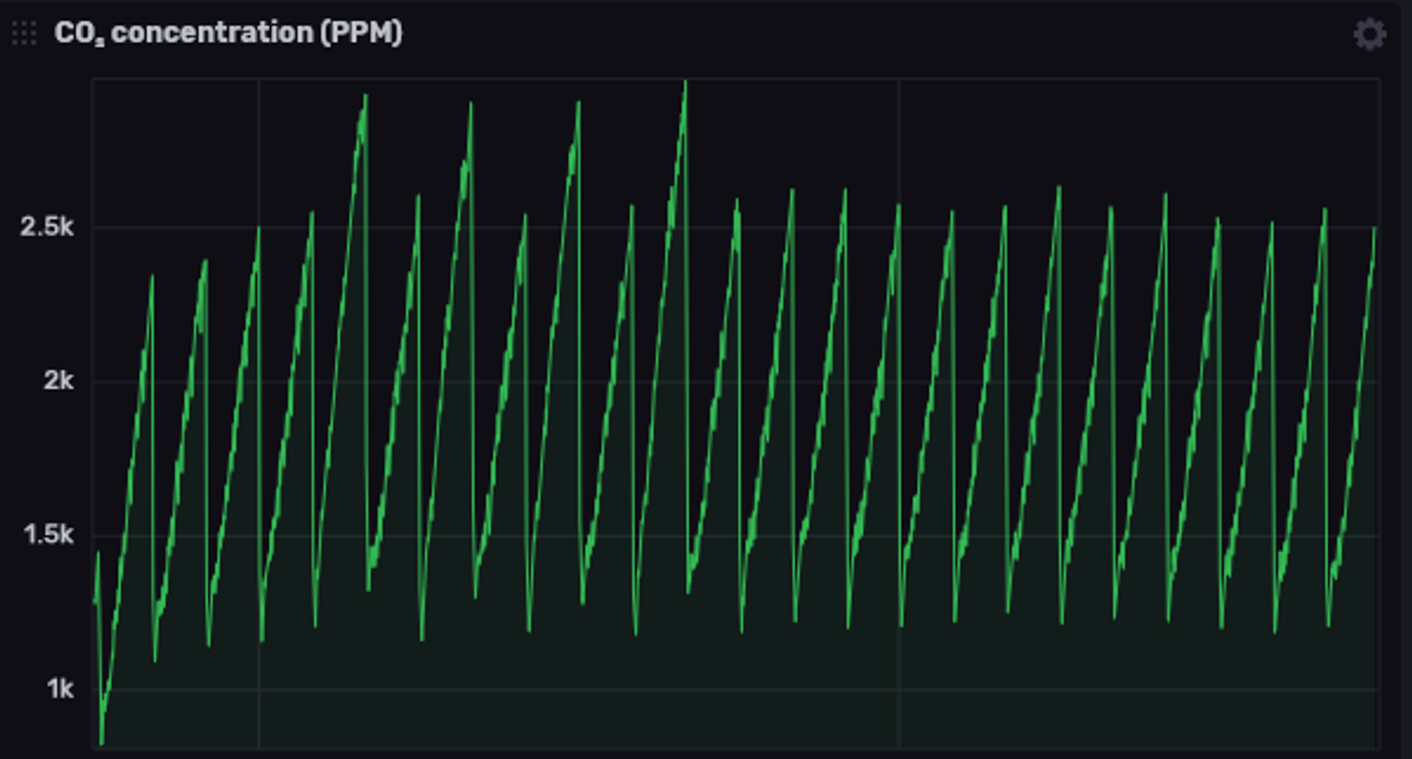
\includegraphics{images/CO2dashboard.png}
    \caption{dioxide of carbon concentration evolution in ppm}
    \label{fig:}
\end{figure} 


\textbf{electrical and flux diagram of the system }

diag diag diag

\textbf{Limit}


\textbf{Future work}

\subsection{Modular environmental control}

This design is quite different from the contolled environment presented just before. 
The aim here is to present an easy way of unpacking a controlled environment. Firstly, the system can be completely dismantled to take up as little space as possible. 

The 3 sections presented above (I.e : the mycelium growth area or growth chamber, the water tank and the electrical panel.) are also found in this system to perform the same functions, but they have different characteristics.

The mycelium growth area,consists of a parallelepiped formed by aluminum profiles for the edges and cushions made from 2 sheets of transparent PVC for the faces. The cushions are inflated with air to provide better thermal insulation. These faces are fixed to the aluminum profile via velco tape. The top and bottom faces (the smallest faces) are in plexiglass. 

This is the part that takes up the most space in traditional designs. Here, all the growth  space is removable. The PVC sides can be deflated and then folded. The aluminum profiles can be removed to take up less space.

The equivalent of the electrical panel is located under the growth space in a small space in an MDF box where the electronics and power supply are located. There are several cables running in and out of this section the main power cable and the power supplies for the sensors and climatic actuators except for the fogger. Inside this hole are the relays and the microcontroller. 

The second special feature of this system is that the water reservoir and the fogger are not located close to the system, but are connected to it by a pipe. The water reservoir constantly generates water aerosol, and humidity is supplied via a fan in the growth space. 
Which makes it easy to centralize several contrasting environments around the tank for testing different cliamatic variables at the same time. 



%%%%%% photo avant apres demontage 
photo avant apres demontage ???????
%%%%%% photo avant apres demontage 

\paragraph{Software}

The data transmission system operates similarly to the approach described in section 3.4.1, but has been streamlined to accommodate additional growth chambers within the same network. Here, a Raspberry Pi serves as the MQTT broker, efficiently managing data flow for multiple chambers. MQTT, or Message Queuing Telemetry Transport, is a publish-subscribe communication protocol designed for lightweight data exchange, making it ideal for managing data between sensors and multiple devices.

In this system, devices can act as either publishers or subscribers. Publishers—such as the various growth systems with sensors monitoring temperature, humidity, and CO₂ levels—send data packets to the broker. Subscribers, such as laptops or user interfaces, can then "subscribe" to specific data streams and receive updates on the conditions within specific chambers.

The broker, by centralizing data flow, allows multiple user devices to monitor data from any sensor without needing to interface with each device individually. This not only simplifies scalability by enabling more growth chambers to be added to the system without extensive reconfiguration, but it also gives users flexibility in viewing specific data streams from particular chambers. Moreover, this setup allows for real-time adjustments, since subscribers can quickly access and act on sensor data, optimizing the control environment for bacterial cellulose or mycelium growth with minimal latency.

\paragraph{Hardware}

As for the sofware, the hardware is basically the same. The major difference comes from the water reservoir. humidity is not pushed through the reservoir and into the growth chamber. humidity is drawn from the reservoir into the growth chamber by a fan. 
This is because in this system, humidity production is centralized, and each controlled envionment unit has its own independent control of the fan that drives the humidity.

The advantage is that even if there are several push chambers, only one fogger is needed, which saves on hardware.

Custom PVC cushions were specifically crafted for this project using a straightforward yet effective approach. By taking two sheets of PVC and welding their edges together, a sealed cushion is created. PVC’s natural adhesiveness simplifies this process—no additional fastening mechanisms are needed to achieve a functional opening.
To incorporate an accessible opening and closing mechanism, the welding process can be left incomplete along a small section of one end, allowing it to act as a “self-sealing” closure. This practical feature makes the cushions easy to fill and empty without additional components, offering versatility in applications ranging from soft support structures to experimental, inflating elements for various settings. Moreover, this design approach leverages PVC’s durability, which enhances resistance to wear, making these cushions reusable and adaptable to different environments.

%%%%%% photo avant apres demontage 
photo coussin ???????
%%%%%% photo avant apres demontage 

\textbf{Electrical and Flow diagram of the system}

diag diag diagggggg

\textbf{Limit}

\textbf{Future work}




















\section{Result}

\begin{figure}[h]
    \centering
    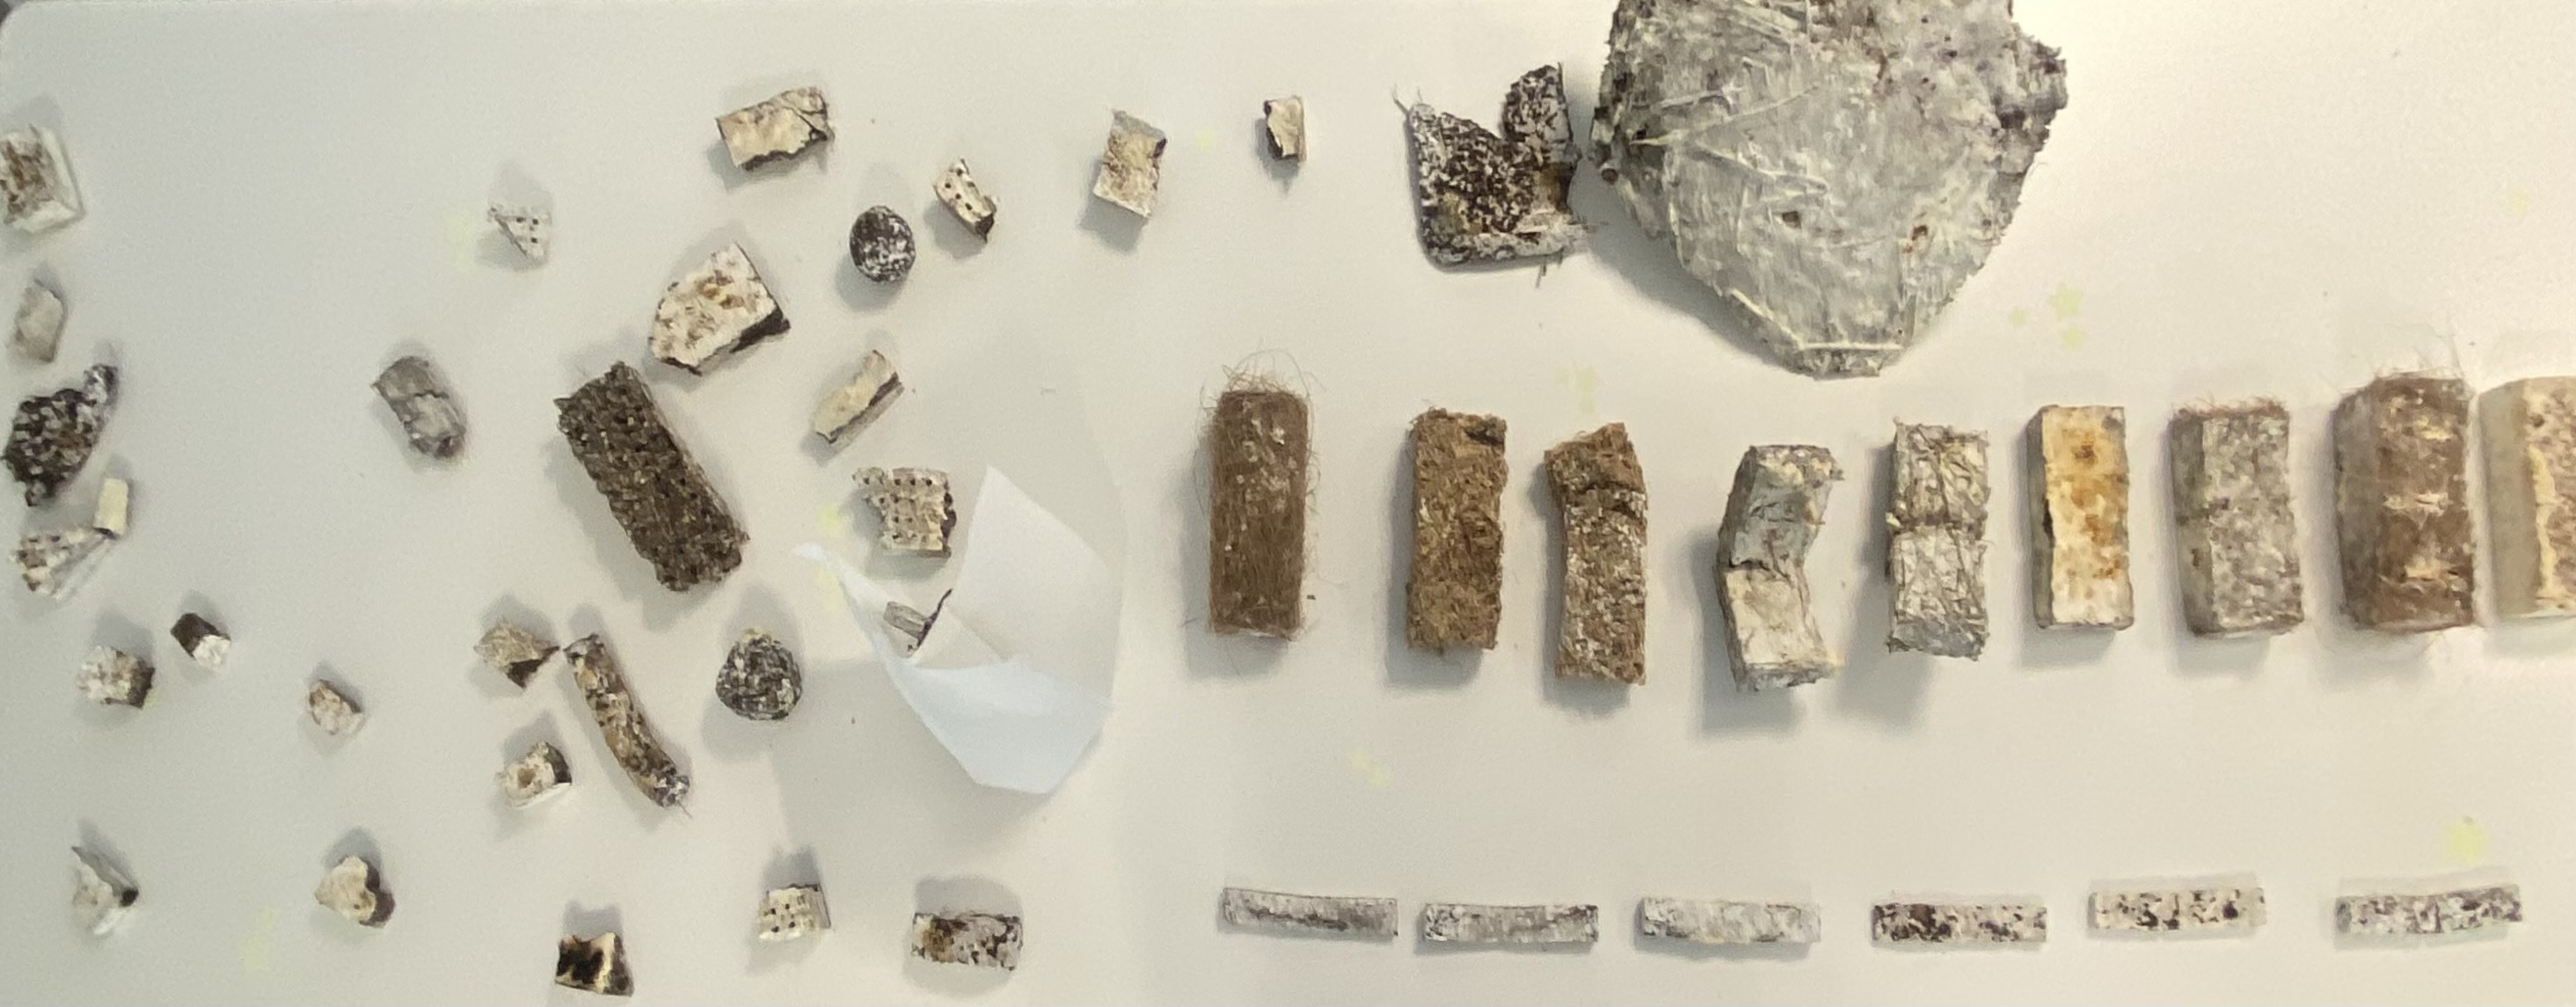
\includegraphics{images/resultMyce.png}
    \caption{Mycelium based materials with different substate}
    \label{fig:mycoproduction}
\end{figure} 

\begin{marginfigure}
    \centering
    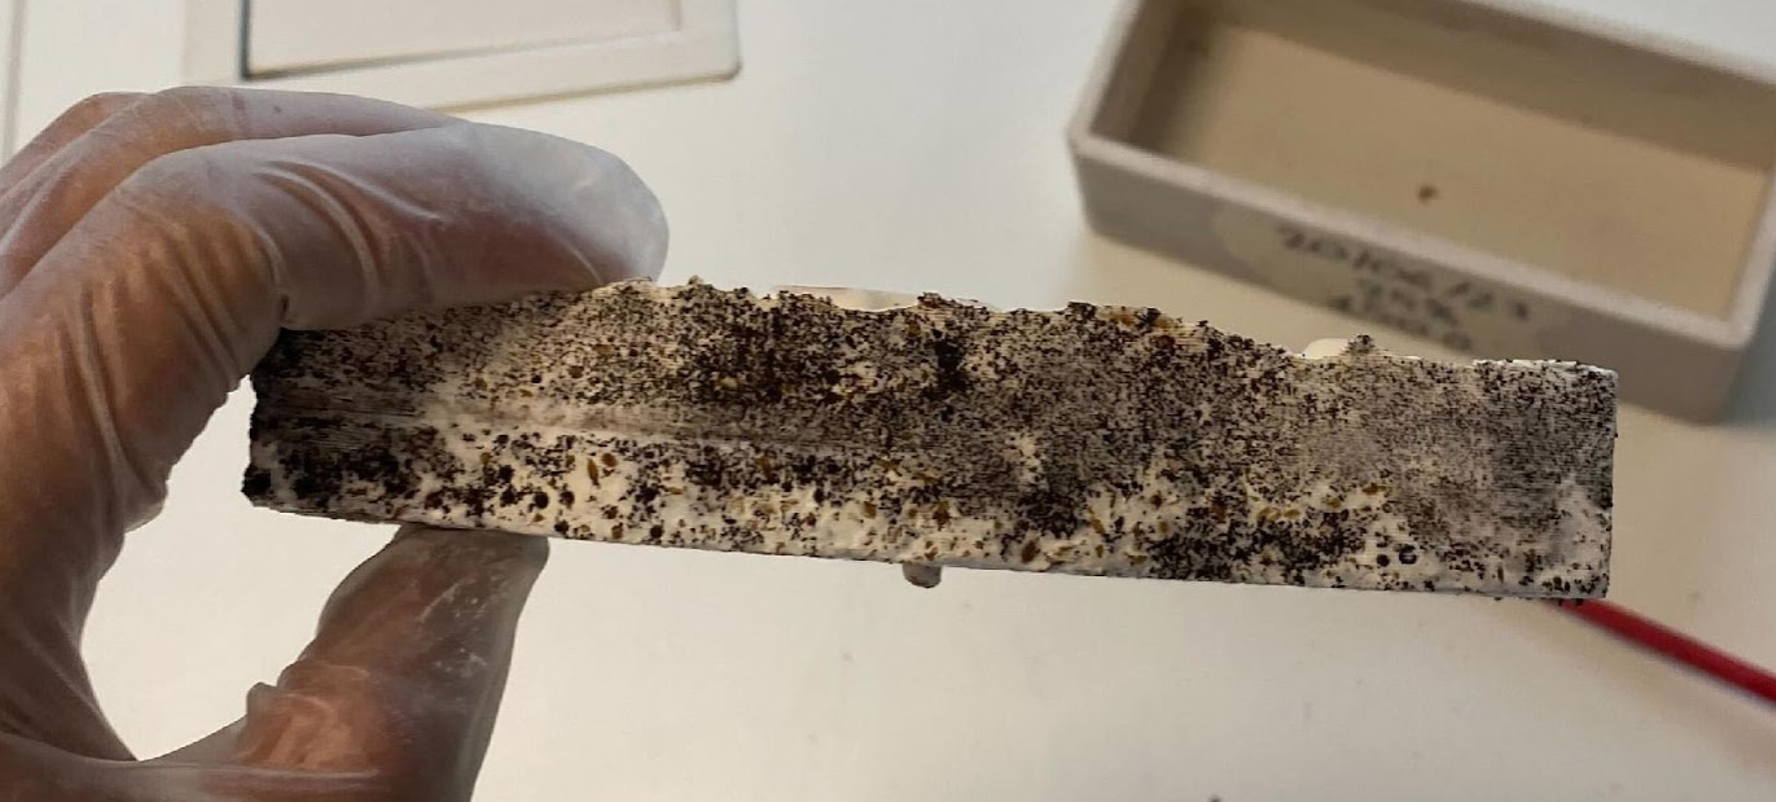
\includegraphics{images/mycoillustration.png}
    \caption{Mycelium based composite preparation}
    \label{fig:illustration myco}
\end{marginfigure}


\begin{figure}[h]
    \centering
    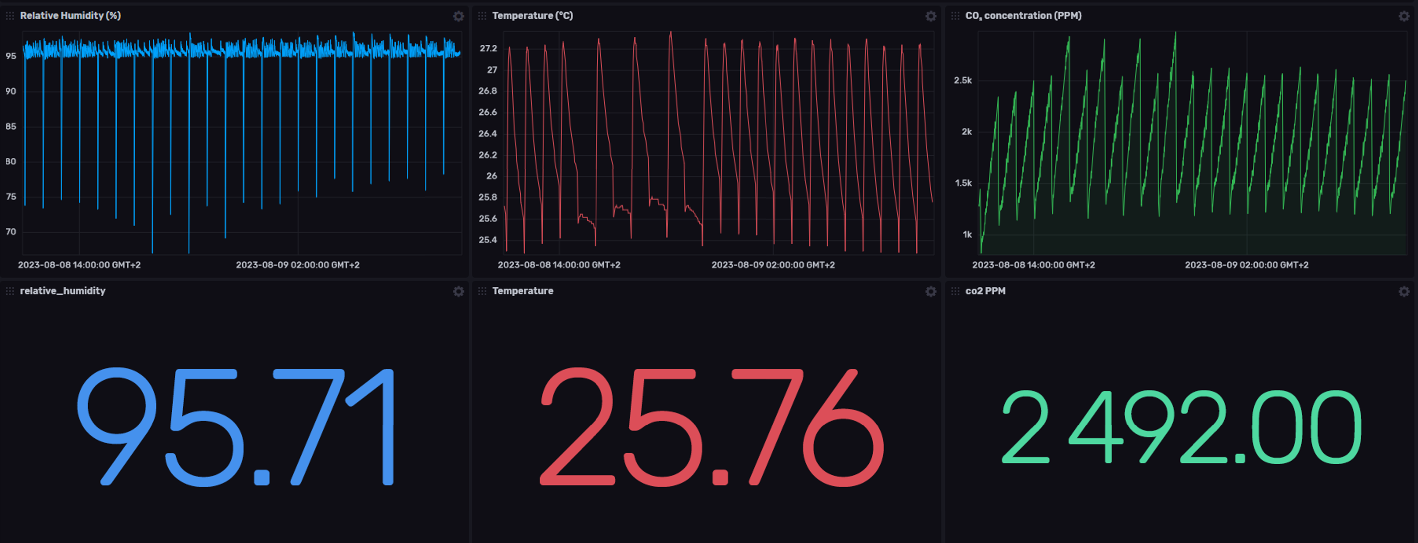
\includegraphics{images/dashboard_all.png}
    \caption{geographic representation of sensors during production of Mycelium biocompisites (Dashboard)}
    \label{fig:dashboardbig}
\end{figure} 

The MBC production cycle takes around 14 days to grow. On the dashboard, you can see the temporal evolution of relative humidity in blue (\%), temperature in red (°C) and carbon dioxide concentration in green (ppm), with the last data taken by the sensors highlighted.

We observe that for relative humidity and temperature the values tend to drop naturally, inverting the carbon dioxide which acts naturally due to the respiration of the fungi. the great variation is due to the renewal of the air which makes take approximately 20\% of relative humidity and 2°C. Given that this is in a short lapse of time and that the system regains the hand quickly this is not a problem for the good development of the mycelium.


\begin{marginfigure}
    \centering
    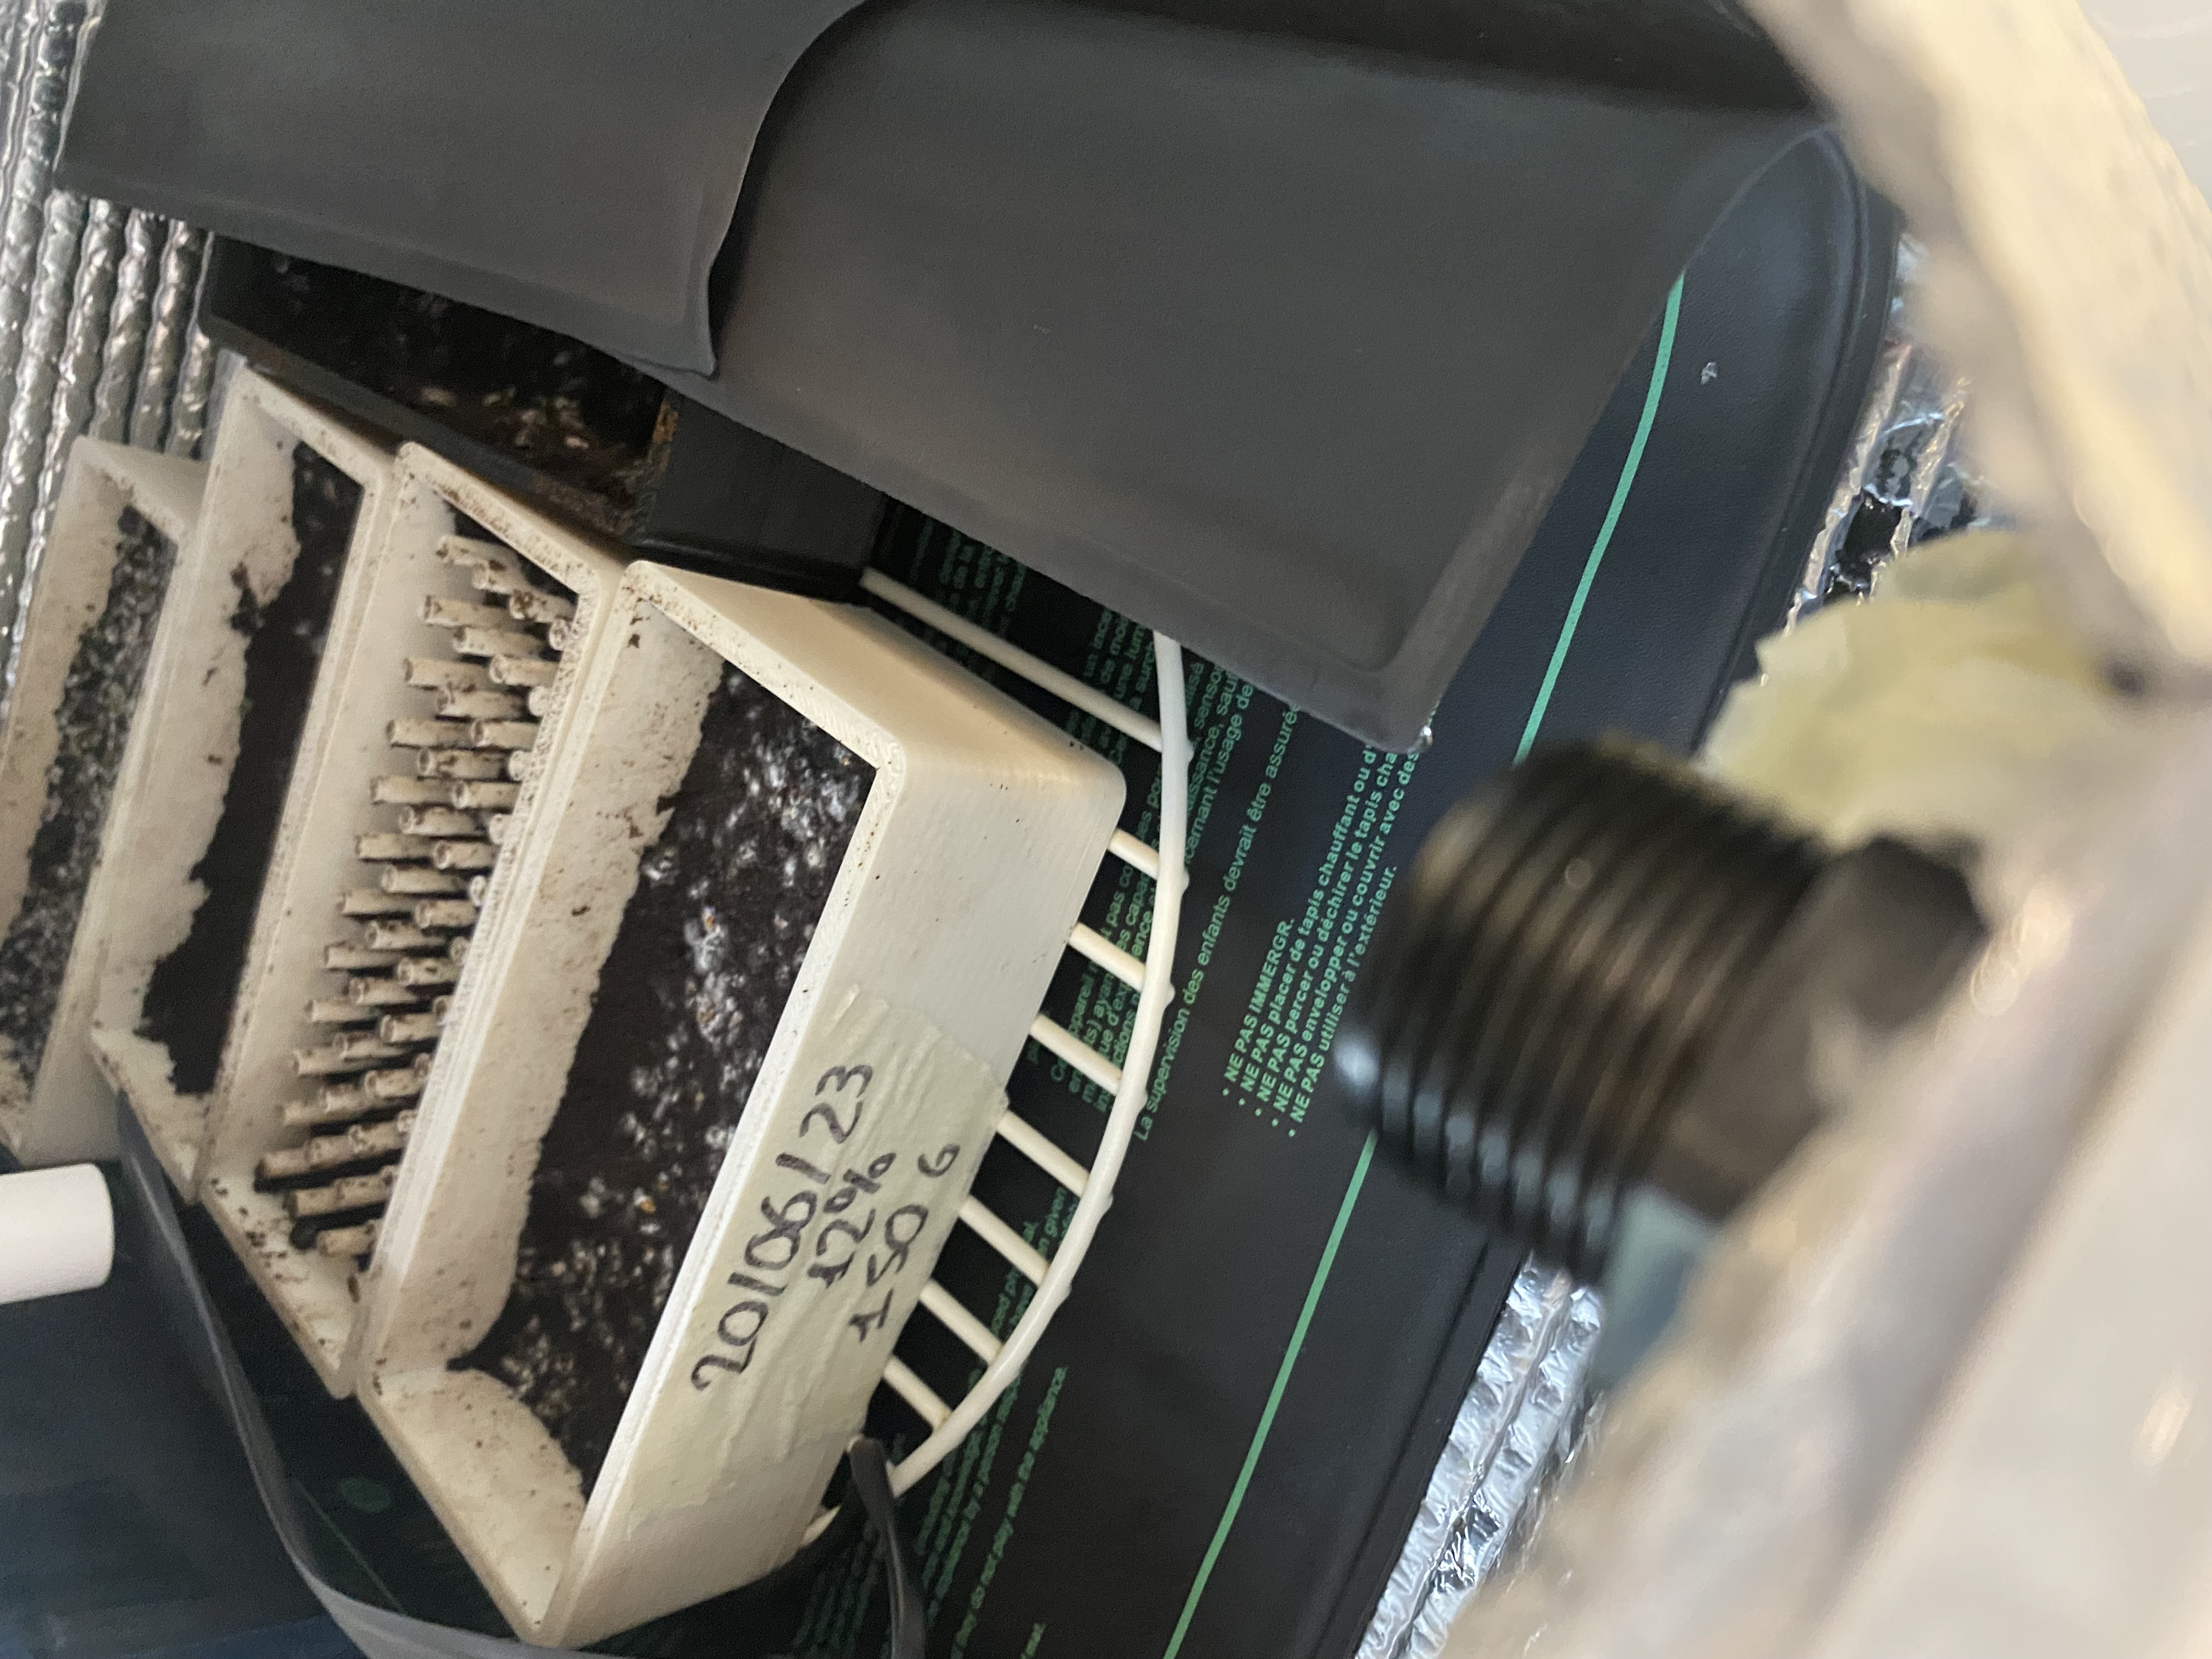
\includegraphics{images/IMG_3172.jpg}
    \caption{Inside Growth chamber}
    \label{fig:insidegrowth}
\end{marginfigure}


\begin{figure}[h]
    \centering
    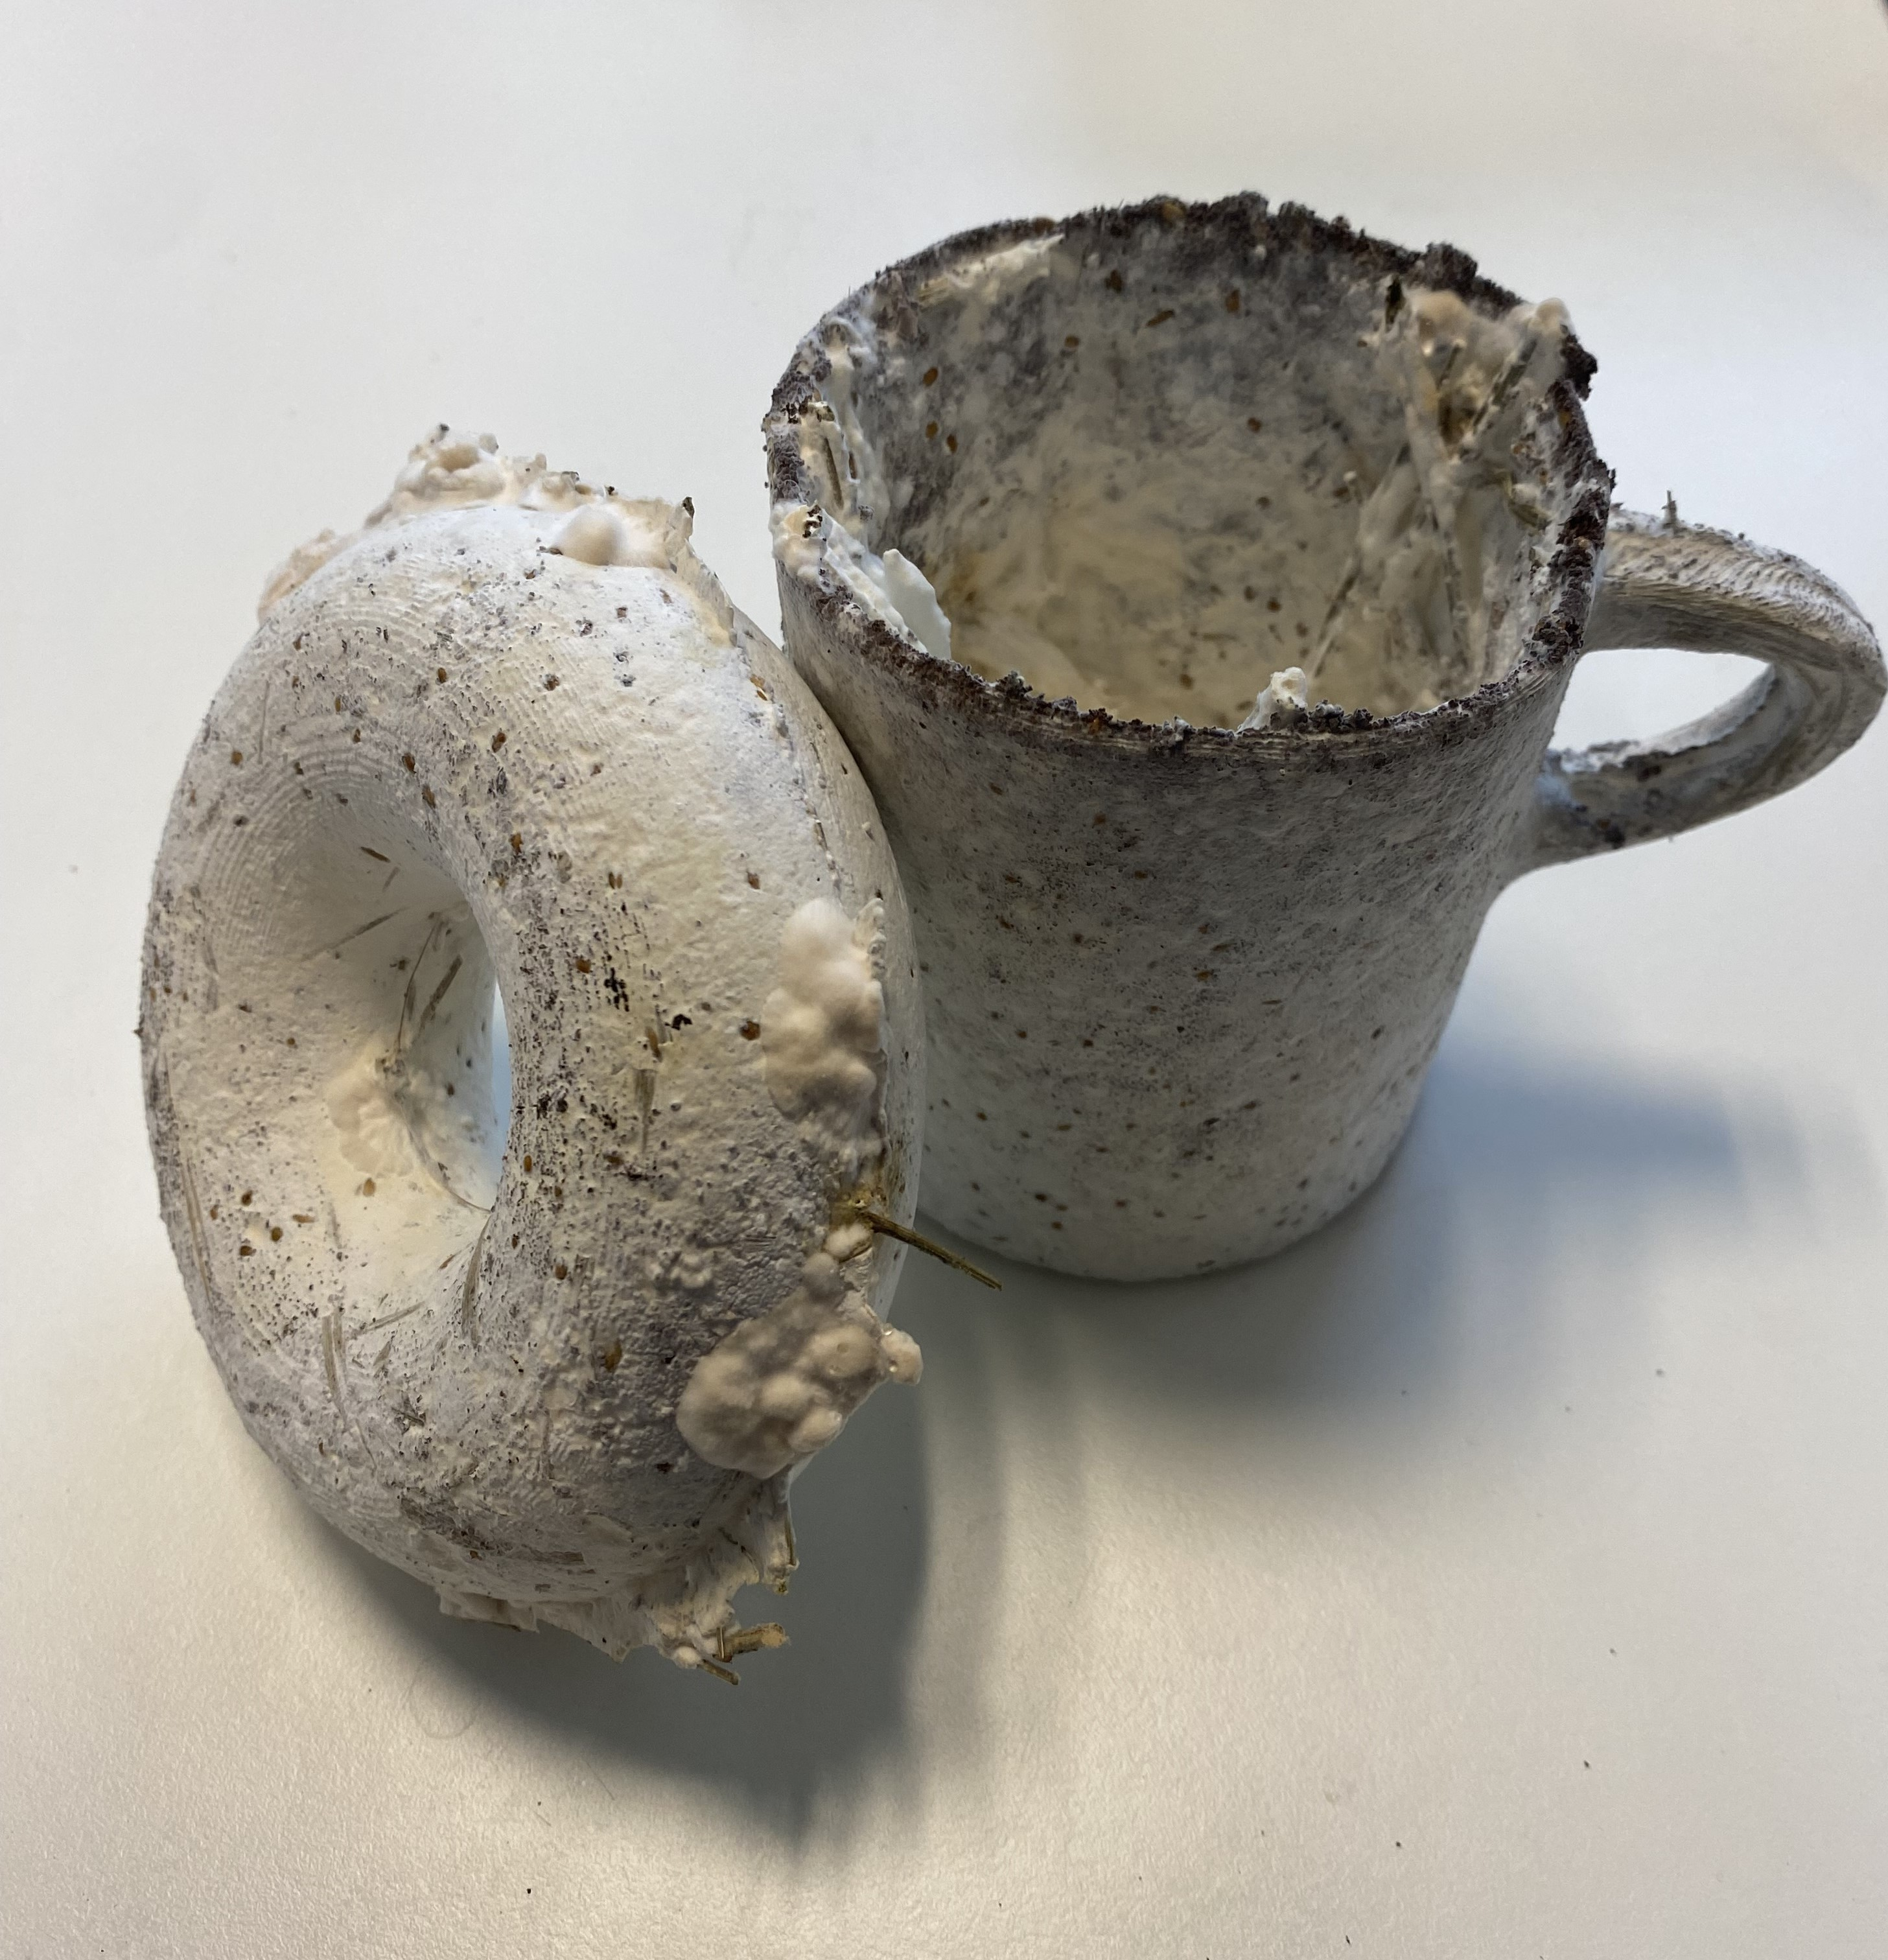
\includegraphics{images/IMG_1838.JPG}
    \caption{}
    \label{fig:Mycemachinne}
\end{figure} 

different recipes have been tested for MCB production 






\subsection{Mechanical test}

experience empirique 
tableau diff substat 